\begin{minipage}{0.49\textwidth}
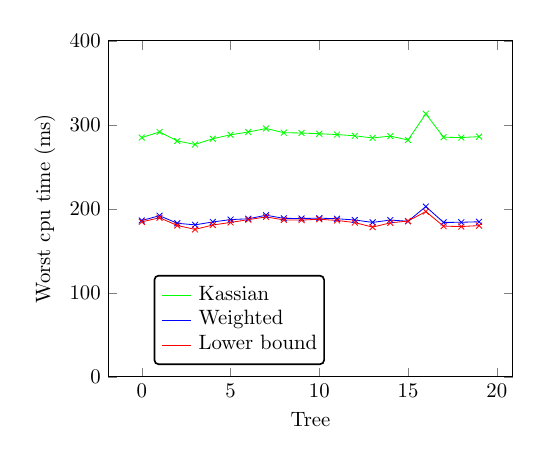
\begin{tikzpicture}[scale=0.75]
  \begin{axis}[ymax=400.75,ymin=0
, xlabel={Tree}, ylabel={Worst cpu time (ms)}]
    \addplot[mark=x, color=green] coordinates { (0,285.241) (1,291.967) (2,281.188) (3,277.046) (4,283.849) (5,288.554) (6,291.871) (7,296.024) (8,291.07) (9,290.673) (10,289.789) (11,288.84) (12,287.317) (13,284.814) (14,286.955) (15,282.34) (16,313.561) (17,285.636) (18,285.266) (19,286.35) };
    \addplot[mark=x, color=blue] coordinates { (0,186.396) (1,192.104) (2,183.067) (3,181.197) (4,184.675) (5,187.452) (6,188.449) (7,192.685) (8,188.957) (9,188.766) (10,189.171) (11,188.499) (12,187) (13,184.14) (14,186.917) (15,185.503) (16,202.992) (17,184.098) (18,184.282) (19,184.882) };
    \addplot[mark=x, color=red] coordinates { (0,184.785) (1,189.678) (2,180.447) (3,175.785) (4,181.032) (5,184.086) (6,187.398) (7,190.672) (8,187.099) (9,186.873) (10,187.898) (11,186.445) (12,183.918) (13,178.478) (14,183.585) (15,185.813) (16,197.031) (17,179.61) (18,179.206) (19,180.3) };
\node[draw=black,thick,rounded corners=2pt,above right=2mm] at (0, 0) {%
  \begin{tabular}{@{}r@{ }l@{}}
    \raisebox{2pt}{\tikz{\draw[green] (0,0) -- (5mm,0);}}&Kassian\\
    \raisebox{2pt}{\tikz{\draw[blue] (0,0) -- (5mm,0);}}&Weighted\\
    \raisebox{2pt}{\tikz{\draw[red] (0,0) -- (5mm,0);}}&Lower bound\\
  \end{tabular}};
  \end{axis}
\end{tikzpicture}
\caption*{Worst cpu time per tree with sites repeats}
\end{minipage}
\begin{minipage}{0.49\textwidth}
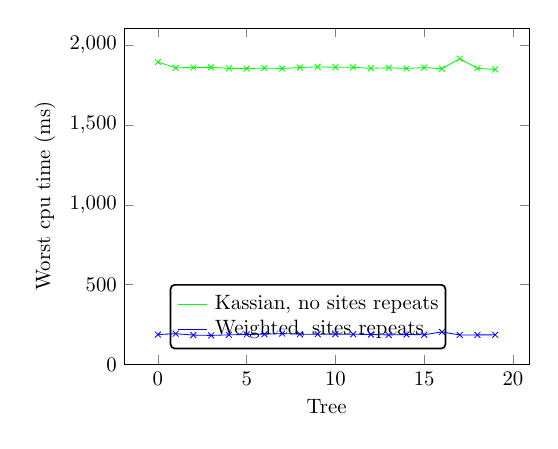
\begin{tikzpicture}[scale=0.75]
  \begin{axis}[ymax=2106.75,ymin=0
, xlabel={Tree}, ylabel={Worst cpu time (ms)}]
    \addplot[mark=x, color=green] coordinates { (0,1894.01) (1,1858.25) (2,1859.56) (3,1860.68) (4,1854.6) (5,1852.93) (6,1856.36) (7,1853.59) (8,1859.64) (9,1863.7) (10,1861.16) (11,1860.8) (12,1854.85) (13,1858.08) (14,1854.01) (15,1859.18) (16,1851.88) (17,1915.23) (18,1854.75) (19,1847.02) };
    \addplot[mark=x, color=blue] coordinates { (0,186.396) (1,192.104) (2,183.067) (3,181.197) (4,184.675) (5,187.452) (6,188.449) (7,192.685) (8,188.957) (9,188.766) (10,189.171) (11,188.499) (12,187) (13,184.14) (14,186.917) (15,185.503) (16,202.992) (17,184.098) (18,184.282) (19,184.882) };
\node[draw=black,thick,rounded corners=2pt,above right=2mm] at (0, 20) {%
  \begin{tabular}{@{}r@{ }l@{}}
    \raisebox{2pt}{\tikz{\draw[green] (0,0) -- (5mm,0);}}&Kassian, no sites repeats\\
    \raisebox{2pt}{\tikz{\draw[blue] (0,0) -- (5mm,0);}}&Weighted, sites repeats\\
  \end{tabular}};
  \end{axis}
\end{tikzpicture}
\caption*{Libpll default implementation against sites repeats implementation}
\end{minipage}
